\documentclass[a4paper,11pt]{article}

%% PREAMBLE %%

% Packages
\usepackage[utf8]{inputenc} % UTF-8 is a good thing I guess
\usepackage[a4paper, total={150mm, 225mm}]{geometry} % use reasonable amount of the page
\usepackage{amsmath}  % allows unnumbered equations
\usepackage{textcomp} % explicitly imported to calm gensymb
\usepackage{gensymb}  % gives degree sign
\usepackage{tikz}     % allows drawing pretty diagrams
\usepackage{pgfplots} % allows graphs and plots
\usepackage{graphicx} % allows images
\usepackage{pdfpages} % allows to import other PDF pages
\usepackage[hidelinks]{hyperref} % allows links to be added in appendix

%\usepackage{tabularx}
%\usepackage{mathtools}
%\usepackage{bm}

%Jono's packages
\usepackage[document]{ragged2e}
\usepackage{subcaption}
\usepackage{fancyhdr}
\usepackage[normalem]{ulem}
\usepackage{colortbl}
\pagestyle{fancy}
\RequirePackage{textcomp}
\RequirePackage{xcolor}
\RequirePackage{listings}
\usepackage[T1]{fontenc}     
\usepackage[framed,numbered]{matlab-prettifier}
\usepackage{epstopdf}
\usepackage{graphicx}

% Titlepage variables
%\title{SA1: Interim Report 1}
%\author{Paul Wernicke (pw444)\\Jonathan Collins (jc2071)}
%\date{May 2020}

\lhead{Week 1 Report}
\rhead{Jonathan Collins \& Paul Wernicke}
\lfoot{jc2071 \& pw444}

%% DOCUMENT %%
\pagenumbering{gobble}
\begin{document}
%\maketitle
\begin{titlepage}
    \begin{center}
 
        \LARGE
        SA1: Aircraft Wing Analysis
        
        \vspace{0.1cm}
        
        \LARGE
        
        Interim Report 1
        
        \vspace{0.4cm}
        
        \large
        
        Jonathan Collins \& Paul Wernicke
        
        \vspace{0cm}
        
        Homerton College
        
        \vspace{0.3cm}
        
        Easter Term 2020
        
        \vspace{0.5cm}
        
        %\large
        
        %\textbf{Abstract}
        
        %\justify
        
        %\normalsize
        %I don't think we really need an abstract.
        %\tableofcontents
        \lstlistoflistings
        \listoffigures
    \end{center}
\end{titlepage}
\pagenumbering{arabic}

\section{Introduction}
This is the introduction. Which we don't need but can use to play around with.


\lstinputlisting[style= Matlab-editor,basicstyle = \mlttfamily,label=script2,
  caption=Exercise 2 script]{build_rhs.m}


\section{Exercise 1}
\begin{figure}[h]
\centering
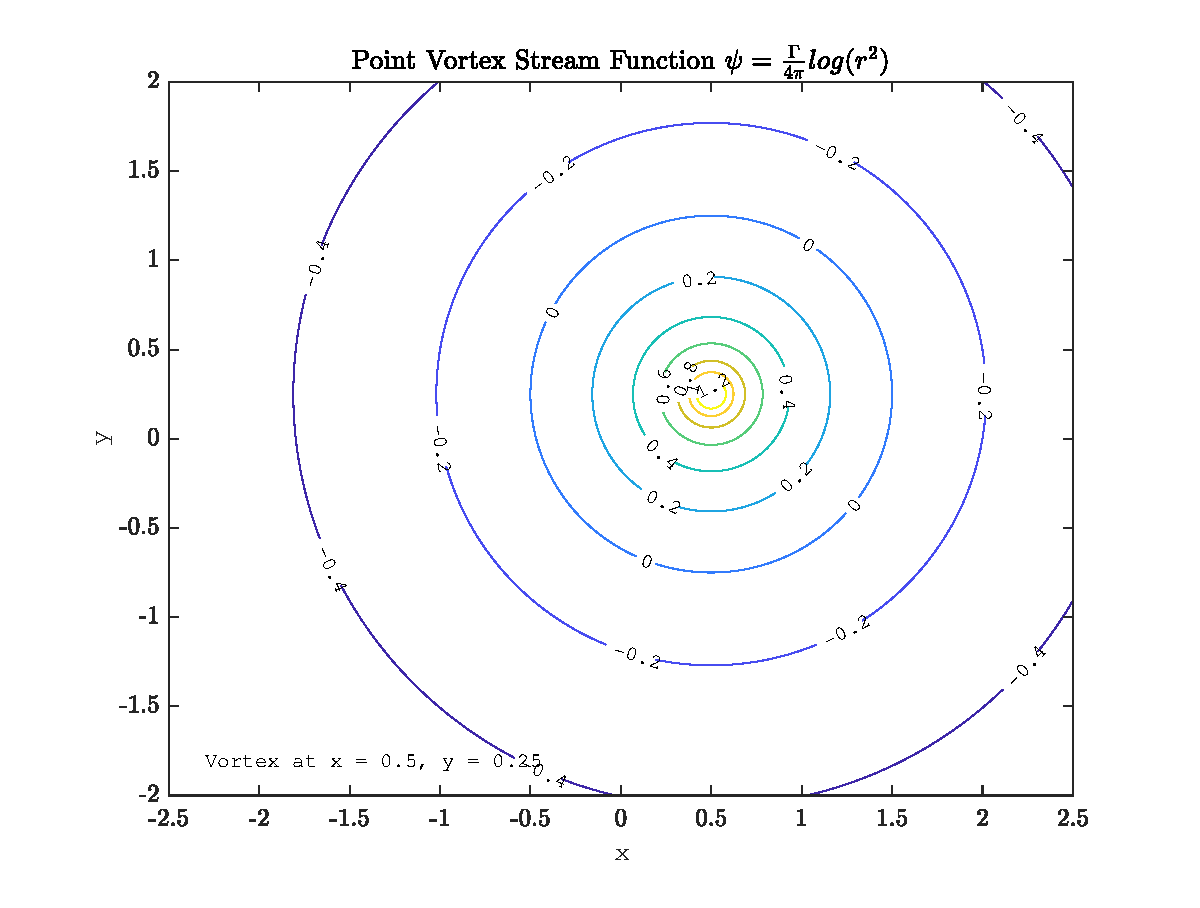
\includegraphics[scale=0.8]{untitled.eps}
\caption{Exercise 1.}
\label{foobar-figure}
\end{figure}

\section{Exercise 2}
% listing of refpaninf.m
\lstinputlisting[style= Matlab-editor,basicstyle = \mlttfamily,label=refpaninf,
  caption=refpaninf.m]{refpaninf.m}

% listing of script
\lstinputlisting[style= Matlab-editor,basicstyle = \mlttfamily,label=script2,
  caption=Exercise 2 script]{Week_1_pw444/exercise2.m}
  
%four contour plots, showing exact and approximate values of fa,fb

\begin{figure}[htbp]
\centering
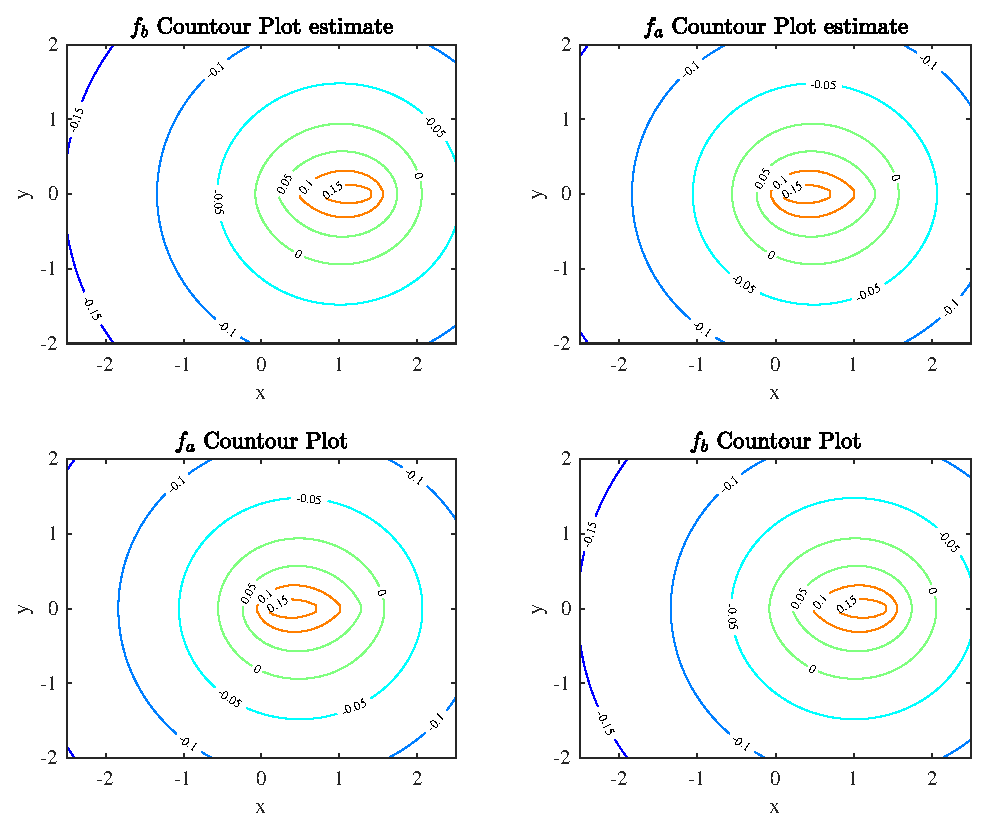
\includegraphics[scale=0.90]{Exercise_2_Contourplots.eps}
\caption{Exercise 1.}
\label{Exercise 2}
\end{figure}

\section{Exercise 3}
% listing of refpaninf.m
\lstinputlisting[style= Matlab-editor,basicstyle = \mlttfamily,label=panelinf,
  caption=panelinf.m]{panelinf.m}
  
\pagebreak

% listing of script
\lstinputlisting[style= Matlab-editor,basicstyle = \mlttfamily,label=script3,
  caption=Exercise 3 script]{Week_1_master/exercise3.m}

% four contour plots, showing exact and approximate values of fa,fb
% contour plot of fa
\begin{figure}[H]
\centering
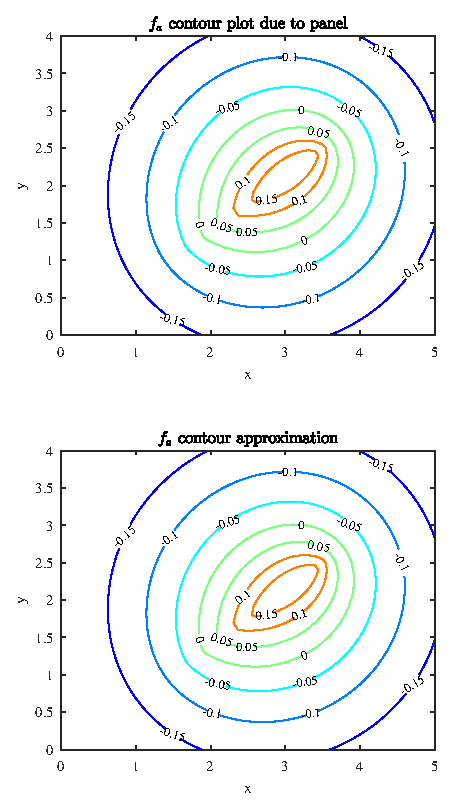
\includegraphics[scale=1.55]{graphs/e3g1.eps}
\caption{Contour plots of $f_a$ for a general vortex-sheet-panel, showing both exact and approximate values}
\label{e3g1}
\end{figure}
% contour plot of fb
\begin{figure}[H]
\centering
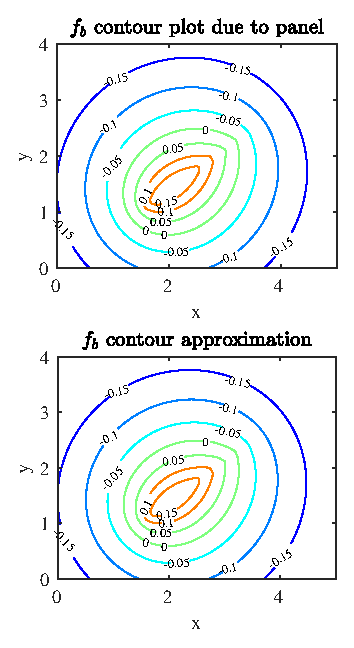
\includegraphics[scale=1.55]{graphs/e3g2.eps}
\caption{Contour plots of $f_b$ for a general vortex-sheet-panel, showing both exact and approximate values}
\label{e3g2}
\end{figure}


\section{Exercise 4}
% listing of script
\lstinputlisting[style= Matlab-editor,basicstyle = \mlttfamily,label=script4,
  caption=Exercise 4 script]{Week_1_master/exercise4.m}
  
% streamline plot
\begin{figure}[H]
\centering
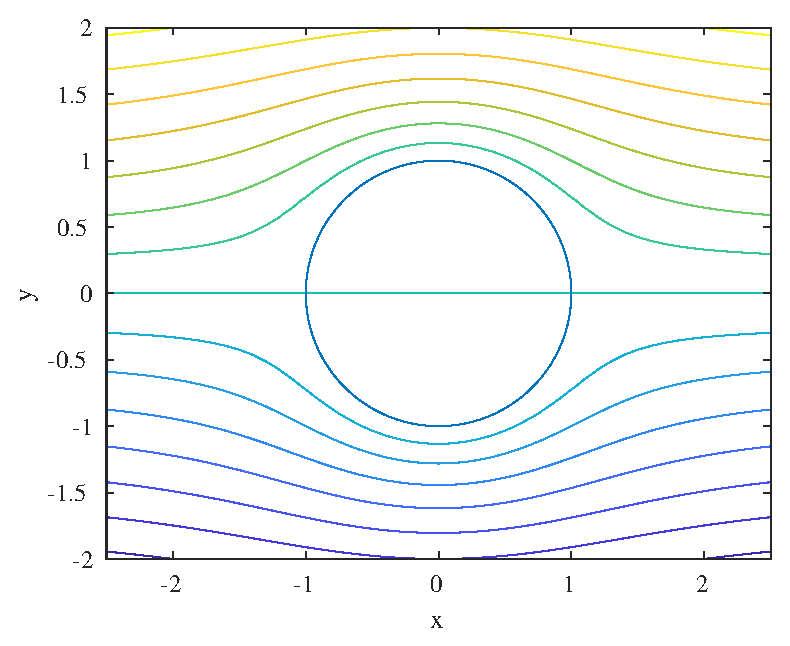
\includegraphics[scale=0.80]{graphs/e4g1.eps}
\caption{Streamline plot over cylinder at $\alpha$ = 0}
\label{e4g1}
\end{figure}

\pagebreak

\section{Exercise 5}
% listing of script
\lstinputlisting[style= Matlab-editor,basicstyle = \mlttfamily,
  caption=Exercise 5 script]{Week_2_master/exercise5.m}

% tabulated separation locations

% graph
\begin{figure}[H]
\centering
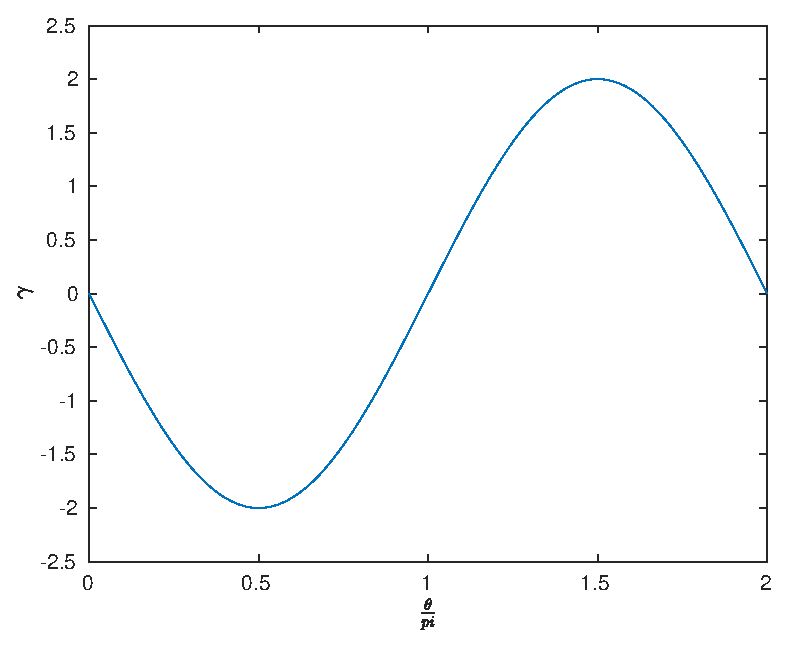
\includegraphics[scale=0.8]{graphs/e5g1.eps}
\caption{kokokok}
\label{e1g1}
\end{figure}

\end{document}